\documentclass[]{article}
\usepackage{amssymb,amsmath}
\usepackage{ifxetex,ifluatex}
\ifxetex
  \usepackage{fontspec,xltxtra,xunicode}
  \defaultfontfeatures{Mapping=tex-text,Scale=MatchLowercase}
\else
  \ifluatex
    \usepackage{fontspec}
    \defaultfontfeatures{Mapping=tex-text,Scale=MatchLowercase}
  \else
    \usepackage[utf8]{inputenc}
  \fi
\fi
\usepackage{ctable}
\usepackage{float} % provides the H option for float placement
\usepackage{graphicx}
% We will generate all images so they have a width \maxwidth. This means
% that they will get their normal width if they fit onto the page, but
% are scaled down if they would overflow the margins.
\makeatletter
\def\maxwidth{\ifdim\Gin@nat@width>\linewidth\linewidth
\else\Gin@nat@width\fi}
\makeatother
\let\Oldincludegraphics\includegraphics
\renewcommand{\includegraphics}[1]{\Oldincludegraphics[width=\maxwidth]{#1}}
\ifxetex
  \usepackage[setpagesize=false, % page size defined by xetex
              unicode=false, % unicode breaks when used with xetex
              xetex,
              colorlinks=true,
              linkcolor=blue]{hyperref}
\else
  \usepackage[unicode=true,
              colorlinks=true,
              linkcolor=blue]{hyperref}
\fi
\hypersetup{breaklinks=true, pdfborder={0 0 0}}
\setlength{\parindent}{0pt}
\setlength{\parskip}{6pt plus 2pt minus 1pt}
\setlength{\emergencystretch}{3em}  % prevent overfull lines
\setcounter{secnumdepth}{0}

\title{Descriptive statistics}
\author{Rapport package team @ https://github.com/aL3xa/rapport}
\date{2011-04-26 20:25 CET}

\begin{document}
\maketitle

\subsection{Description}

This template will return descriptive statistics and frequency table of
a categorical variable.

\subsection{\emph{gender} (``Gender'')}

The dataset has \emph{709} observations with \emph{673} valid values
(missing: \emph{36}) in \emph{gender} (``Gender''), which seems to be a
qualitative variable.

\subsubsection{Base statistics}

\ctable[pos = H, center, botcap]{lllll}
{% notes
}
 & \textbf{Cumul.
N} & \textbf{Cumul. \%}
\ML
male & 410 & 60.9212 & 410 & 60.9212
\\\noalign{\medskip}
female & 263 & 39.0788 & 673 & 100
\\\noalign{\medskip}
Total & 673 & 100 & 673 & 100
\LL
}

\subsubsection{Barplot}

\href{3a46554ee29cd4dfe45dda5016464658-hires.png}{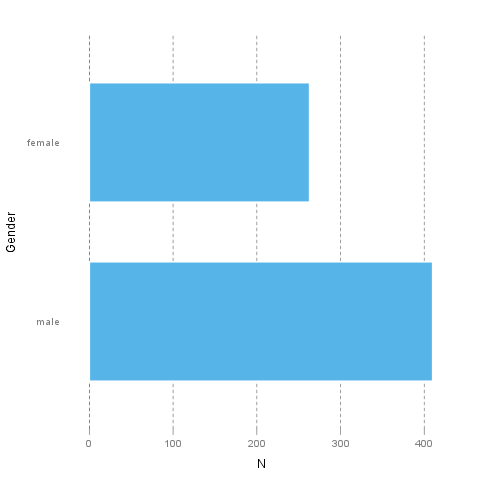
\includegraphics{3a46554ee29cd4dfe45dda5016464658.png}}

It seems that the highest value is \emph{2} which is exactly 2 times
higher than the smallest value (\emph{1}).

The most frequent value is \emph{male}.

\subsection{Description}

This template will return descriptive statistics and frequency table of
a categorical variable.

\subsection{\emph{dwell} (``Dwelling'')}

The dataset has \emph{709} observations with \emph{662} valid values
(missing: \emph{47}) in \emph{dwell} (``Dwelling''), which seems to be a
qualitative variable.

\subsubsection{Base statistics}

\ctable[pos = H, center, botcap]{lllll}
{% notes
}
 & \textbf{Cumul.
N} & \textbf{Cumul. \%}
\ML
city & 599 & 90.4834 & 599 & 90.4834
\\\noalign{\medskip}
small town & 33 & 4.9849 & 632 & 95.4683
\\\noalign{\medskip}
village & 30 & 4.5317 & 662 & 100
\\\noalign{\medskip}
Total & 662 & 100 & 662 & 100
\LL
}

\subsubsection{Barplot}

\href{a370513c6bd94251e700ff5fea9dd33f-hires.png}{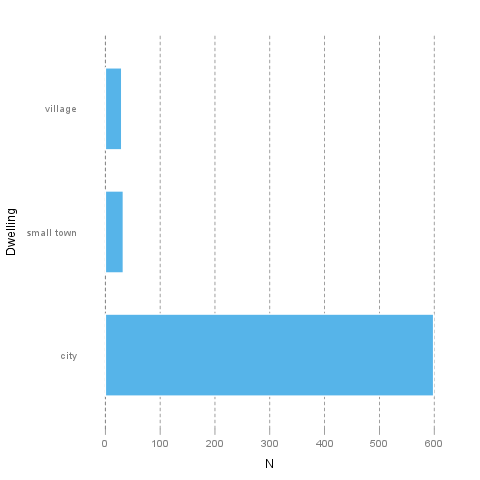
\includegraphics{a370513c6bd94251e700ff5fea9dd33f.png}}

It seems that the highest value is \emph{3} which is exactly 3 times
higher than the smallest value (\emph{1}).

The most frequent value is \emph{city}.

\begin{center}\rule{3in}{0.4pt}\end{center}

This report was generated with \href{http://www.r-project.org/}{R}
(2.14.0) and \href{http://al3xa.github.com/rapport/}{rapport} (0.2) in
0.769 sec on x86\_64-unknown-linux-gnu platform.

\begin{figure}[htbp]
\centering

\includegraphics{images/logo.png}
\caption{}
\end{figure}

\end{document}
